\section{Methods}
\label{sec:methods}

\begin{comment}
Here you explain how you’ve solved the problem
in our case

SITUATION: Problem X is very important because . . .
COMPLICATION: In tackling problem X, related work failed in doing Y
PROPOSAL: To partly tackle Y, we make N contributions [list of contributions]

X = organizational moral misalignment
Y = incorporating different perspectives

we solve the problem of incorporating different perspectives
so we explain how we did it
\end{comment}

To address the challenge of incorporating diverse organizational perspectives into ethical decision-making, we propose a software tool designed to support company decision-makers.
This section describes the design and operation of the tool we developed to simulate organizational moral reasoning using role-based AI agents.
We first explain the intended use of the tool and the type of input it receives from the user. We then describe how the system simulates the reasoning of three organizational roles using artificial intelligence agents. Finally, we detail how the tool generates a structured summary from these simulated perspectives and delivers it to the user.
Figure \ref{fig:impl} summarises the tool architecture.

\subsection{Tool Purpose and Use Context}

While ethical dilemmas in corporate contexts often involve conflicting viewpoints (such as operational feasibility, long-term impact, and normative values), real-world decision processes frequently lack mechanisms to systematically consider these different angles before a decision is made.
A software tool offers three primary advantages in this context. First, it provides structured access to a plurality of perspectives that may otherwise be inaccessible due to hierarchical, departmental, or cultural barriers. Second, it enables consistent and scalable reasoning support that can be applied to a wide range of cases without requiring additional personnel or meetings. Third, by relying on artificial intelligence agents prompted to emulate distinct organizational roles, the tool encourages users to reflect more critically on the trade-offs and value conflicts embedded in each dilemma.
The intended users are decision-makers in organizations: particularly those at the executive or senior management level, who are often required to resolve complex ethical scenarios quickly, under uncertainty, and without comprehensive stakeholder input. Our tool aims to enrich this decision process by making invisible perspectives explicit, in a structured and neutral form.

\subsection{Dilemma Input}

The user begins by inputting a moral dilemma into the tool.
In our context, a dilemma is defined as a scenario describing a realistic organizational situation that involves an ethically relevant conflict. A dilemma includes a brief narrative containing background information (the description of a scenario, including the roles of the stakeholders involved, the context in which the decision must be made, and any relevant constraints) followed by one or more open-ended questions requiring the user to take a position or justify a course of action.
By formulating the dilemmas in this way, we ensure that the tool operates on rich, ambiguous inputs that reflect the types of challenges decision-makers face in real-world contexts.

\subsection{Role-based Agents}

\paragraph{Persona Prompts}{
  Once the dilemma is submitted, the tool initiates an internal simulation involving three artificial intelligence agents, powered by large language models (LLMs). Each agent is assigned a fixed organizational role: a chief executive officer, an engineer, and an ethicist. These roles were selected to reflect three core domains of organizational reasoning: strategic authority, technical feasibility, and moral evaluation.
  To ensure that each role-based agent reliably reflects its assigned organizational role, we design tailored prompts that define the agent's responsibilities, values, and communication style. Each prompt specifies the agent's professional identity within a fictional mid-sized company and outlines the reasoning strategies it should apply when responding to the dilemma.
  These role-specific prompts (referred to as \textit{personas}) are not simply character sketches; they are designed to elicit structurally distinct forms of reasoning that mirror real-world organizational tensions.
  The CEO agent (Prompt \ref{prompt:ceo}) is instructed to prioritize long-term organizational success, brand reputation, and strategic decision-making, with a focus on risk-benefit trade-offs and pragmatic leadership. The engineer agent (Prompt \ref{prompt:engineer}) emphasizes feasibility, technical integrity, operational constraints, and potential implementation risks. The ethicist agent (Prompt \ref{prompt:ethicist}) centers its reasoning on moral principles, stakeholder rights, and social responsibility, often challenging decisions that may appear effective but raise ethical concerns.
}

\paragraph{Task}{
  The simulation starts by instantiating the three role-based agents and dispatching a common task to each of them individually. To construct the task, we embed the user-provided dilemma into a common task template (Prompt \ref{prompt:task}). This template instructs an agent to read the dilemma and respond in approximately 300 words, providing their reasoning, thoughts, and opinions. Each agent receives this same structured task, but interprets and responds to it according to the role-specific instructions defined in their \textit{persona} prompt.
}

\paragraph{Topology}{
  Rather than engaging in freeform debate, the agents operate within a standardized discussion topology. The agents respond independently, without direct interaction with one another. This design choice reflects our goal of faithfully simulating distinct organizational viewpoints without introducing conversational dynamics such as persuasion, alignment, or social conformity that may occur in natural group discussions. This \textit{Ensemble} structure ensures clarity and prevents conversational drift, allowing each agent to contribute a distinct, coherent viewpoint. This topology is not designed to reach consensus, but rather to expose areas of convergence and divergence in how each role interprets the dilemma.
}

\subsection{Summary Output}

\paragraph{Moderator Agent}{
  Once the three role agents have expressed their positions, a fourth agent, the Moderator, is activated using a separate instruction set: the \textit{combination instructions} (Prompt \ref{prompt:combination}). This prompt defines the moderator's objective as supporting a human decision-maker by analyzing and summarizing the agents' individual outputs in a structured, accessible format. The moderator is explicitly instructed to identify and present the core tensions raised in the responses, areas of agreement and disagreement among the agents, and a list of practical considerations that the user should address in their own justification. The moderator's tone is constrained to be neutral, direct, and free of technical or philosophical jargon, to ensure accessibility and minimize framing bias.
}

\paragraph{Summary Structure}
The moderator thus produces a summary that is composed of three parts: (1) a list of points on which the agents agreed, providing a sense of organizational alignment; (2) a list of disagreement areas and competitive priorities, revealing underlying tensions or conflicting viewpoints between roles; (3) a set of practical questions or considerations that the user is encouraged to reflect on when making their own decision.
This design emphasizes cognitive support over persuasive framing, aiming to augment the user's moral reflection without biasing the outcome.
The purpose of this output is not to recommend a specific course of action, but to broaden the user's moral reasoning by foregrounding perspectives they may overlook. By surfacing both consensus and conflict among roles that typically shape corporate decision-making, the tool helps users critically examine their own intuitions, mitigate personal blind spots, and produce more structured, well-reasoned responses.

\begin{figure}[h]
  \centering
  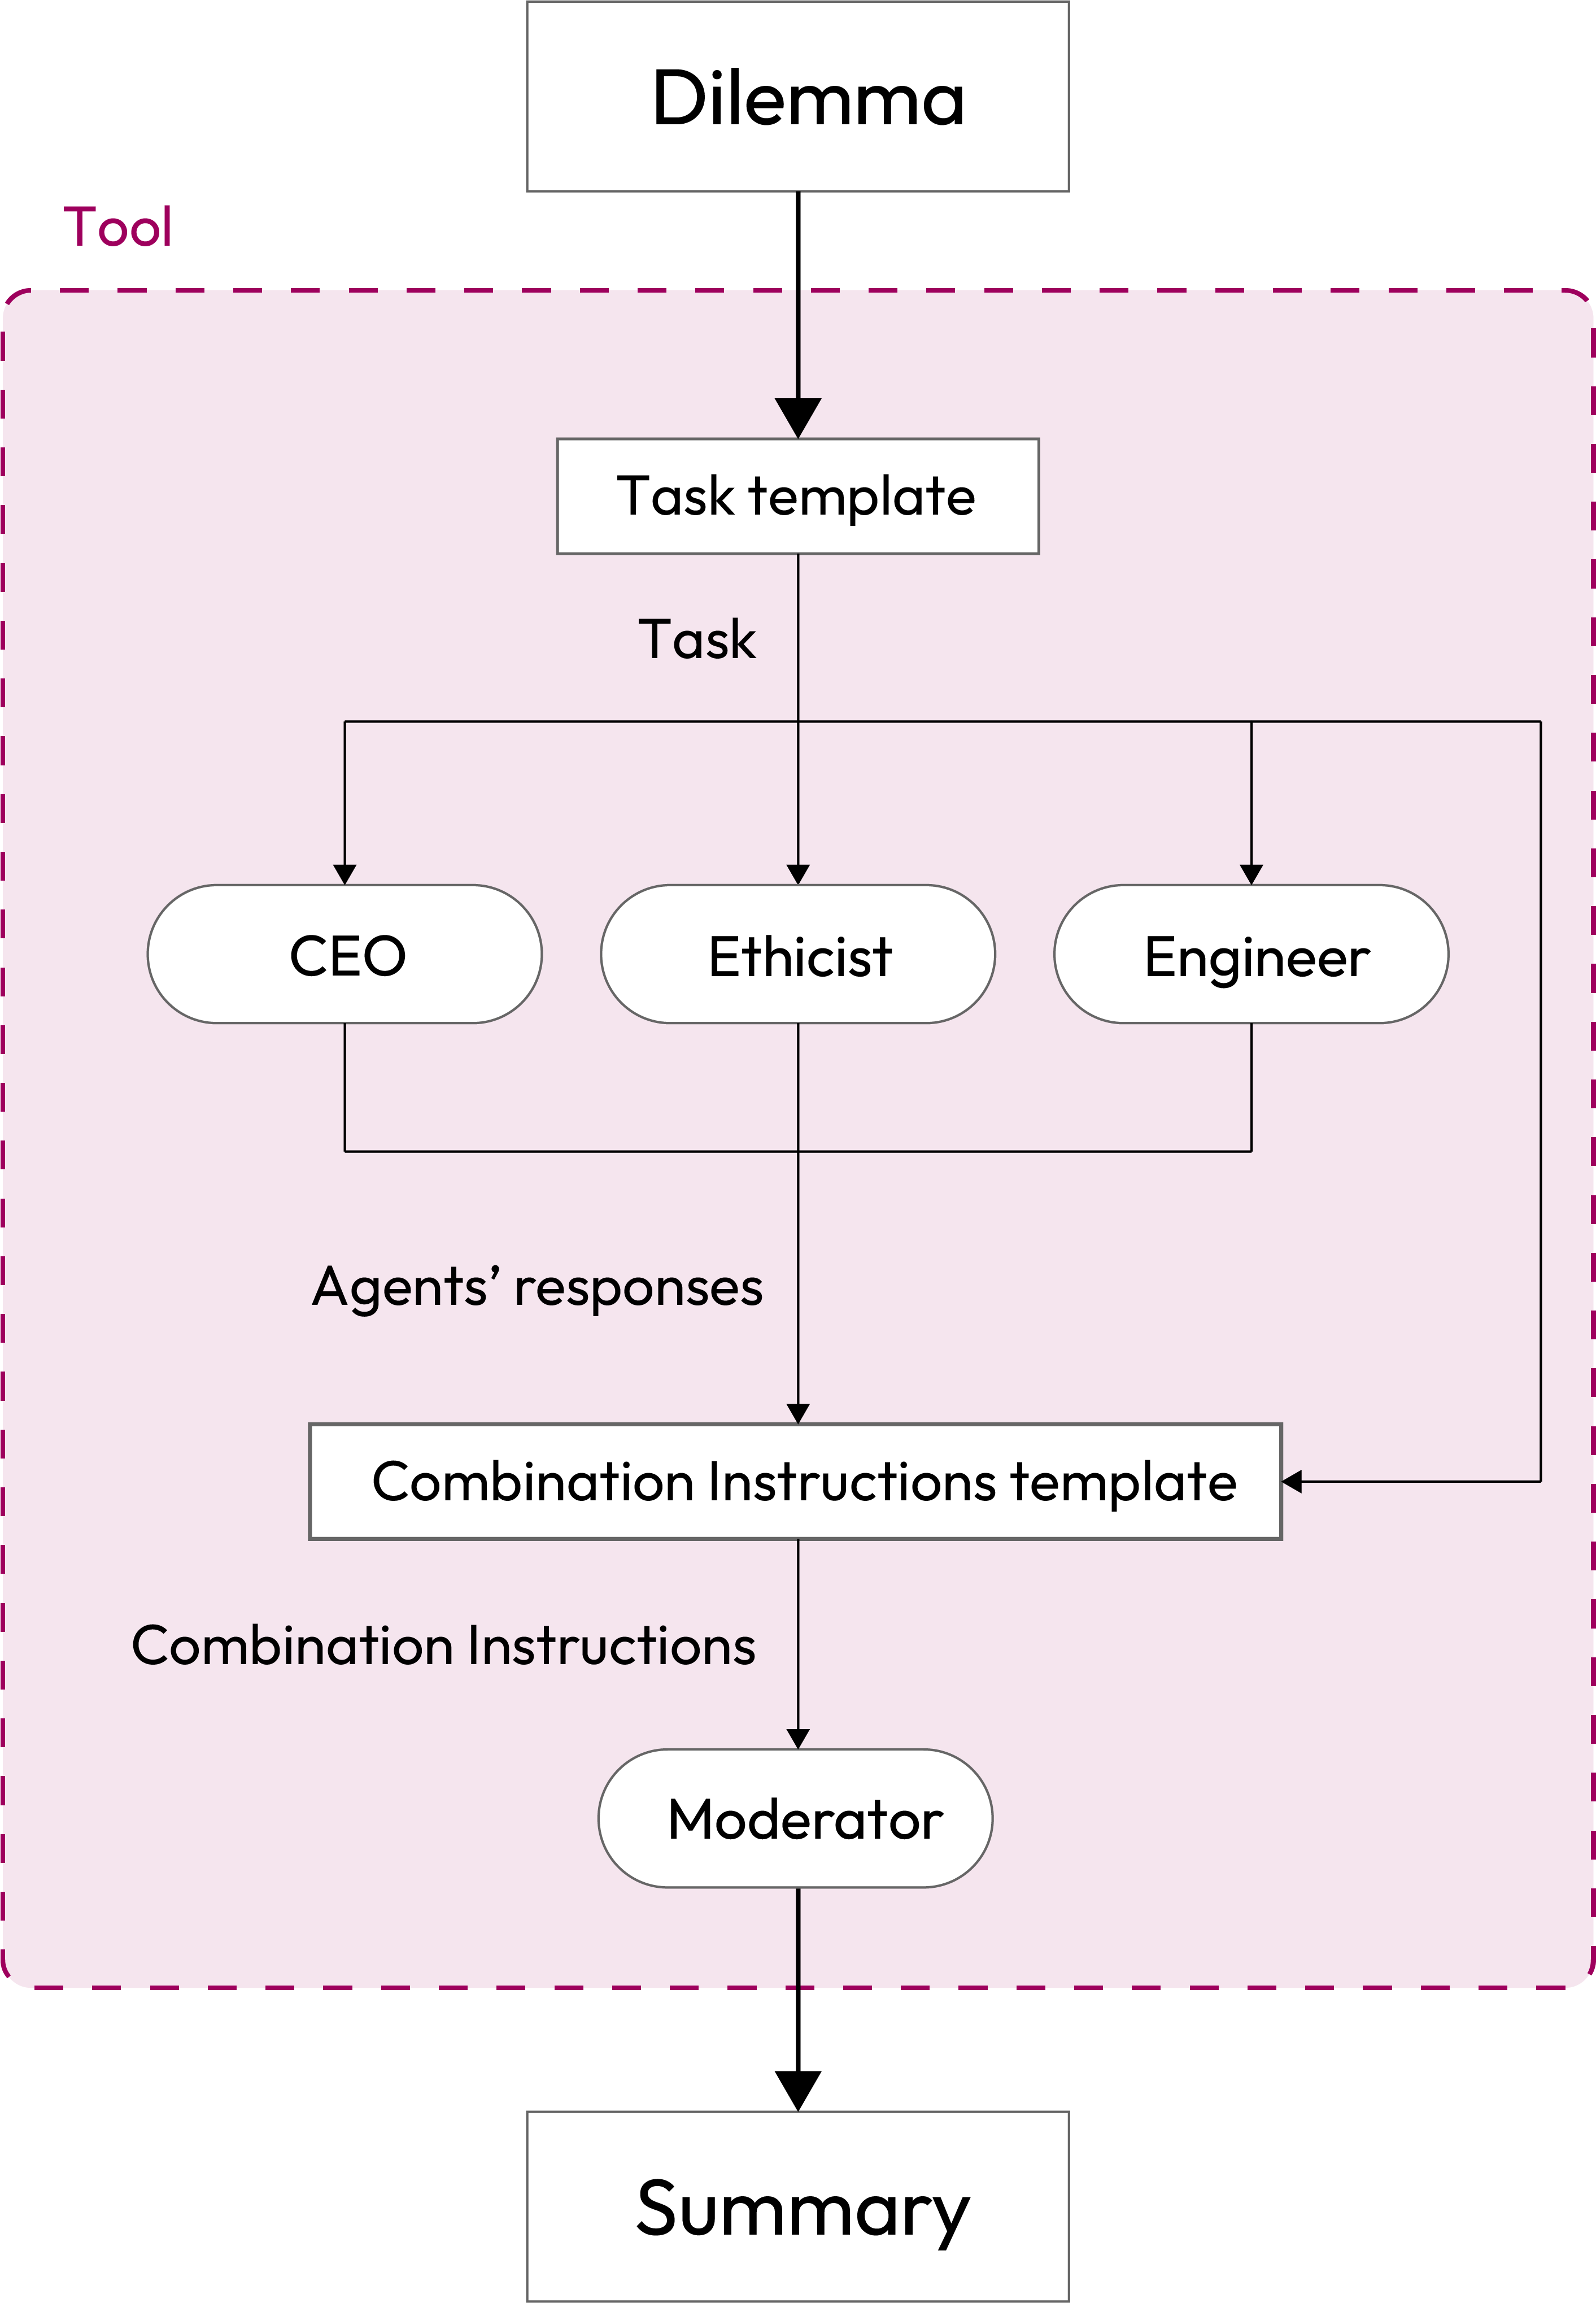
\includegraphics[width=\linewidth]{impl}
  \caption{Overview of the tool's architecture. The user provides a moral dilemma, which is embedded into a task template and submitted independently to three artificial intelligence agents representing the roles of CEO, ethicist, and engineer. Each agent responds based on a predefined persona prompt. The agents' responses are then passed to a moderator agent via a combination instructions template. The moderator analyzes the content and produces a structured summary highlighting agreement, disagreement, and suggested considerations for the user.}
  \Description{Overview of our tool's architecture.}
  \label{fig:impl}
\end{figure}
